\DocumentMetadata{lang=en-US, pdfversion=2.0, pdfstandard=ua-2, tagging=on}
% Build with: docs/build.sh   (TinyTeX lualatex, three passes, for a tagged PDF/UA-2 file)
\documentclass[11pt, letterpaper]{article}

\usepackage[margin=0.9in]{geometry}
\usepackage{fontspec}
\setmainfont{texgyrepagella}[Extension=.otf, UprightFont=*-regular,
  BoldFont=*-bold, ItalicFont=*-italic, BoldItalicFont=*-bolditalic]
\setsansfont{texgyreheros}[Extension=.otf, UprightFont=*-regular,
  BoldFont=*-bold, ItalicFont=*-italic, BoldItalicFont=*-bolditalic]
\setmonofont{Inconsolatazi4}[Extension=.otf, UprightFont=*-Regular,
  BoldFont=*-Bold, Scale=0.92]
\usepackage{microtype}
\usepackage{xcolor}
\definecolor{navy}{HTML}{1F2E4A}
\usepackage{graphicx}
\graphicspath{{figures/}{images/}}
\usepackage{booktabs}
\usepackage{tabularx}
\usepackage{enumitem}
\setlist{itemsep=2pt, topsep=4pt}
\usepackage{needspace}
\usepackage[font=small, labelfont=bf, skip=6pt]{caption}
\usepackage{titlesec}
\titleformat{\section}{\sffamily\Large\bfseries\color{navy}}{\thesection}{0.6em}{}
\titleformat{\subsection}{\sffamily\large\bfseries\color{navy}}{\thesubsection}{0.6em}{}
\titlespacing*{\section}{0pt}{16pt}{6pt}
\titlespacing*{\subsection}{0pt}{12pt}{4pt}
\usepackage{hyperref}
\hypersetup{pdftitle={fleetwatch: one screen for many Claude Code sessions},
  pdfauthor={Daniel Pittman}, colorlinks=true, linkcolor=navy, urlcolor=navy}
\makeatletter
\g@addto@macro{\UrlBreaks}{\do\-}
\makeatother

% A figure never lands above the point in the text where it is placed, so it
% always follows the paragraph that cites it. Floats also keep source order.
\usepackage{flafter}
% Let a page carry two figures, or one with a few lines of text, before LaTeX
% gives up and sends a figure to a page of its own.
\renewcommand{\topfraction}{0.9}
\renewcommand{\bottomfraction}{0.8}
\renewcommand{\textfraction}{0.1}
\renewcommand{\floatpagefraction}{0.8}
\setcounter{totalnumber}{3}
\setlength{\emergencystretch}{2em}


% Command lines and file contents, set small in the mono face. Plain verbatim
% keeps the tagged build simple: each block is one structure element.
\newenvironment{code}{\par\smallskip\small}{\par\smallskip}
\newcommand{\cmd}[1]{\texttt{#1}}
% A screenshot set a little wider than the text, centred, so 120 terminal columns
% print near 7 pt. The makebox keeps the overhang out of the overfull-box count.
% Usage: \shot[trim left bottom right top]{alt text}{file}
\NewDocumentCommand{\shot}{O{0 0 0 0} m m}{%
  \makebox[\linewidth][c]{\includegraphics[width=1.06\linewidth, trim=#1, clip, alt={#2}]{#3}}}

\begin{document}

\begin{center}
  
\includegraphics[width=0.9in, alt={The fleetwatch logo: a radar scope on a navy
    rounded square, its sweep lighting one amber blip among teal ones.}]{fleetwatch-logo}\par
  \vspace{6pt}
  {\sffamily\bfseries\huge fleetwatch\par}
  \vspace{4pt}
  {\large One screen for many Claude Code sessions, and a memory for each of them\par}
  \vspace{8pt}
  Daniel Pittman \quad·\quad November 2026 \quad·\quad
  \href{https://github.com/daniel-pittman/fleetwatch}{\nolinkurl{github.com/daniel-pittman/fleetwatch}}\par
\end{center}

\vspace{4pt}
\noindent\emph{AI-use disclosure: This overview was written with AI assistance. An AI
assistant (Claude, by Anthropic) helped draft the prose, draw the architecture figure and
check each command shown here by running it against the code, and fleetwatch itself was
built with Claude Code under my direction. The design and the working practices described
here are mine. The screenshots are rendered by the app from its built-in demo, a fleet of
fictional sessions, and the logo was generated with Google's Gemini (Nano Banana) image
model.}

\section{Why I built it}

I run a lot of Claude Code sessions at once. Each one has its own job: a feature in one
repository, a code review in another, a budget spreadsheet, a documentation site. Some
are \emph{personas}, named sessions that watch a team's Slack channel on a timer and help
the people in it. On a busy day that is a dozen terminals or more.

Two things go wrong at that scale. The first is attention. A session that needs me asks in
its own terminal, and the question waits there until I happen to look. A permission prompt
can hold a session still for an hour. A date a session promised to remind me about is in
its scrollback, not in front of me. The second is continuity. A long session compacts its
context and loses facts it knew yesterday, and a finished session is hard to find three
months later, when I no longer remember which folder it ran in.

fleetwatch is my answer to both, in three layers:

\begin{enumerate}
  \item \textbf{The board}: one screen of every session and what it needs from me, one
    hotkey away from any terminal.
  \item \textbf{Session memory}: a searchable, scrubbed index of each session's own
    transcript and its reference folders, so a session can look up what compaction dropped.
  \item \textbf{The search engine} underneath, a plain library that works on any folder of
    documents.
\end{enumerate}

The board needs only Python and Textual. The memory layers are optional extras. Everything
runs on one machine, with no service and no account.

\section{The board}

The board opens on \emph{Needs you} (Figure~\ref{fig:board-needs-you}). It lists the
sessions that are waiting on me, and only those. A session shows up there for one of three
reasons: it is stuck on a permission prompt, it holds questions for me, or it owns one of
my to-dos that is overdue, due today or still has no date. A stuck session sorts first,
since it blocks work, then a session with something overdue. Space opens a row to its
numbered questions and items, and Enter jumps to that session's terminal tab.

\begin{figure}[htbp]
  \centering
  \shot{The Needs you tab of the
    demo board. The header reads: 4 questions, 1 stuck, 1 overdue, 1 due today, 3 working,
    1 quiet. Four sessions are open, each with its state. Billing API, persona Robin, is stuck on a prompt for 7
    minutes and has two questions, one from its helper. Release Notes has an overdue item in
    red: send the 2.4 release notes to the partner list. Checkout Flow has two questions, the
    oldest waiting 3 hours. Newsletter has an item due today. Below them an Indexes section lists three indexes
    that need a look: site-docs is stale, release-history failed its last refresh, and
    advising-notes was refused by the protection check. A small radar mark floats over the
    bottom right corner with one amber blip.}{board-needs-you}
  \caption{Needs you, with every row open. The radar mark in the bottom right corner keeps its
    one blip amber while anything here needs me.}
  \label{fig:board-needs-you}
\end{figure}

The header counts what needs me, and the radar mark floating over the bottom right corner
turns its one blip amber while anything does. It is decoration: everything it signals is
also written out. On a terminal under 32 rows or 100 columns it is hidden. Each row also
says whether its session is working, idle or gone quiet, as on the Sessions tab. A last
section, \emph{Indexes}, appears when a memory index failed its last refresh, failed its
protection check or went stale.

Four more tabs sit beside it (Figure~\ref{fig:board-sessions}). \emph{Your to-dos} puts my
own items from every session in one list: undated items first, since they need a date, then
dated ones, overdue first. Everything else a session mentions, such as milestones, meetings
and its own internal work, folds into one closed \emph{Also noted} section. \emph{Sessions}
lists every live session by state: working, gone quiet and idle. A session that promised to
report every 30 minutes and missed it is \emph{gone quiet}, which is usually the first sign
that a persona's loop has stopped. Helper sessions (subagents, worktree lanes, background
runs) are found by process ancestry and counted on their parent's row, so ten helpers do not
bury the session that started them.

\begin{figure}[htbp]
  \centering
  \shot{The Your to-dos tab of the demo board. Three of my
    items are listed by date: Nov 9, overdue, send the 2.4 release notes to the partner
    list, from Release Notes; today, approve the autumn newsletter draft, from Newsletter;
    Nov 21, review supplier feed changes, from Inventory Sync. A closed section, Also
    noted, holds four more.}{board-todos}\par\medskip
  \shot{The Sessions tab of the demo board. Working: Search
    Tuning (Rowan), Docs Site (Piper), and Billing API (Robin), stuck on a prompt with 1
    helper. Gone quiet: Inventory Sync, quiet, expected every 30 minutes, updated 1.6 hours
    ago. Idle: Newsletter, Checkout Flow (Sage) and Release Notes (Piper).}{board-sessions}
  \caption{Your to-dos (top) and Sessions (bottom). The tab bar along the bottom carries a
    count on every tab.}
  \label{fig:board-sessions}
\end{figure}

\emph{Resume} is for later (Figure~\ref{fig:board-resume}). It lists the sessions I gave a
name that are stopped or parked, and leaves out the thousands of unnamed helper transcripts.
Each row says where the session left off, read from its last status file: what it was
working on, my next dated item and how many questions it still held. Parking a session adds
a note on top (\cmd{fleetwatch park --note "waiting on the new price list"}). Enter resumes
the session in this terminal and \cmd{o} opens it in a new iTerm2 window. fleetwatch refuses
to resume a session that is still running, since two processes on one transcript would
corrupt it, and it refuses a launch folder that no longer exists rather than start the
session somewhere else. From a shell, \cmd{fleetwatch resume pricing} finds the same session
by part of its name.

\begin{figure}[htbp]
  \centering
  \shot{The Resume tab of the demo board. A Parked section
    holds Pricing Page, last active Nov 11, folder ~/code/storefront/pricing, parked with the
    note: waiting on the new price list from finance. Under it: was: new annual plans on the
    pricing page, next: Nov 15 check the price list again, status 20 hours ago. The row is
    open and shows the folder and session ID. Below, Status Page, Nov 9, ~/code/site/status,
    was: moving the status page to the new host, 1 question, status 2 days ago. The footer
    lists the keys: Enter resume here, o new window, / find, p park, u unpark.}{board-resume}
  \caption{Resume, with one parked session open to its folder and session ID.}
  \label{fig:board-resume}
\end{figure}

The last tab, \emph{Indexes} (Figure~\ref{fig:board-indexes}), is a health check on the
session memory, grouped by trust group. Each index shows when it last refreshed and
whether that worked, whether it is stale, whether the protection check passes for a
protected group, and its counts of exchanges and files. It never shows what is inside an
index, and it never refreshes one. \cmd{y} copies a search command for the highlighted
index.

\begin{figure}[htbp]
  \centering
  \shot{The Indexes tab of the demo board, grouped by trust group. archive: release-history,
    a session index whose last refresh failed (build) 40 minutes ago, 530 exchanges, 41
    files. ferpa: advising-notes, refreshed 20 minutes ago, protection refused (settings),
    77 exchanges, 12 files. team: site-docs, a plain index refreshed 5 hours ago and marked
    stale, 212 files; storefront-sessions, refreshed 14 minutes ago, 1842 exchanges, 96
    files. The hint line offers y to copy a search command.}{board-indexes}
  \caption{Indexes: status and counts only.}
  \label{fig:board-indexes}
\end{figure}

Two more keys get a lot of use. \cmd{/} (or Ctrl-K) finds any live session by part of its
name or persona, and Enter jumps to it. \cmd{G} groups every tab by project folder, using
rules in \cmd{groups.toml}, and \cmd{m} moves a session to another group.

\subsection{The overlay}

The feature I use most is the hotkey window. On macOS with iTerm2, one command installs it:

\begin{code}
\begin{verbatim}
fleetwatch iterm install
\end{verbatim}
\end{code}

That writes an iTerm2 Dynamic Profile: a hotkey window on Control-Shift-F, full width at the
top of the screen, floating over every Space. I press Control-Shift-F from anywhere and the
board is there. Enter on any row raises that session's tab, in whichever window and Space
it lives, and Control-Shift-F hides the board again. The board is one keystroke from every
terminal, and a question never waits long for me to notice it.

\subsection{Try it}

\cmd{fleetwatch --demo} runs the live board on a fictional fleet in a temporary folder:
seven sessions in two groups, one helper and two sessions to resume. Every screenshot in
this document comes from it. It never reads or writes my own files, and Enter on a Resume
row resumes nothing. \cmd{fleetwatch --demo --once} prints a plain snapshot instead, and
\cmd{--json} prints the full data for scripts.

\section{How a session reports: the status file}

The board reads what Claude Code already records: its registry of running sessions,
\cmd{claude agents --json}, and the transcripts. That tells it which sessions are alive and
whether one is waiting on a prompt. It cannot tell what a session is working on, or what it
needs me to decide. For that, each session writes one small status file.

A session writes it by piping JSON to \cmd{fleetwatch write-status}
(Figure~\ref{fig:status}). The command finds the calling session by walking up the process
tree to the first process with a registry entry, stamps the session's name, ID and the time,
and writes the file atomically. The file is keyed by the session ID, so a renamed session
keeps its file. Table~\ref{tab:fields} lists the fields; only the ones a session sends are
written.

\begin{figure}[htbp]
\begin{code}
\begin{verbatim}
$ echo '{"persona": "Robin",
         "working_on": "adding retry to the invoice job",
         "questions": ["Should refunds over the limit need a second approver?"],
         "upcoming": [{"what": "Approve the retry policy", "due": "2026-11-20",
                       "kind": "todo", "yours": true}]}' | fleetwatch write-status
wrote ~/.claude/state/fleetwatch/billing-api.json

$ cat ~/.claude/state/fleetwatch/billing-api.json
{
 "session": "Billing API",
 "sessionId": "5e551011-0000-4000-8000-0000000000aa",
 "updated": "2026-11-11T22:55:11-05:00",
 "persona": "Robin",
 "working_on": "adding retry to the invoice job",
 "questions": ["Should refunds over the limit need a second approver?"],
 "upcoming": [{"what": "Approve the retry policy", "kind": "todo",
               "yours": true, "due": "2026-11-20"}]
}
\end{verbatim}
\end{code}
  \caption{A session reports its status. \cmd{write-status} adds the session's name, ID and
    the time; the file is shown here with its lists folded onto one line.}
  \label{fig:status}
\end{figure}

\begin{table}[htbp]
  \centering\small
  \caption{The fields a session sends to \cmd{fleetwatch write-status}.}
  \label{tab:fields}
  \begin{tabularx}{\linewidth}{@{}>{\raggedright\arraybackslash}p{2.6cm}X@{}}
    \toprule
    Field & What it carries \\
    \midrule
    \cmd{working\_on} & One line on the current task. \\
    \cmd{questions} & Decisions only I can make: a string, or \cmd{\{"q": ..., "since": ...\}}
      so the board can show how long one has waited. \\
    \cmd{upcoming} & Dated items: \cmd{what}, \cmd{due}, \cmd{kind} and \cmd{yours}. The kinds
      are \cmd{deadline}, \cmd{deploy}, \cmd{meeting}, \cmd{milestone}, \cmd{todo} and
      \cmd{checkin}. \cmd{"yours": true} marks something I must do myself; only those reach
      Needs you. \\
    \cmd{persona} & The persona's name, shown beside the session's. \\
    \cmd{cadence\_min} & How often the session promises to report. A missed report moves it
      to Gone quiet. \\
    \bottomrule
  \end{tabularx}
\end{table}

\cmd{write-status} is strict on purpose. An item with a key it does not know is refused with
a hint (``unknown key \cmd{when}; did you mean due?''). An item of mine with no date is
refused with a suggestion: when the real date is unknown, use a \cmd{checkin} item dated
for the day to look again. The error goes back to the session that wrote it, so the session
learns the format the first time it gets it wrong, and nothing quietly disappears because it
was filed under the wrong key.

I ask every session to write its status whenever its questions change and at the end of any
turn that leaves work running. That instruction lives in my global \cmd{CLAUDE.md}, so every
session follows it without being told again.

\section{Personas: a practice the board supports}

A persona is a long-running session with a name and a job. Mine watch a team's channel on a
timer, answer what they can, keep the team's work from stalling, and bring me the questions
they should not answer alone. A student team gets a persona that knows its repository and its
backlog; a service gets one that watches its pull requests and its deploys.

fleetwatch does not run personas. It makes a handful of them manageable:

\begin{itemize}
  \item The persona's name shows beside the session's, as in \emph{Billing API (Robin)}, so I
    know who is asking.
  \item A persona writes its status on every firing, with its \cmd{cadence\_min}. When its loop
    stops (the session closed, the machine slept), the session moves to Gone quiet with
    ``expected every 30 min'' and I notice within one cycle.
  \item Its questions reach Needs you the moment they are written, and the radar turns amber.
  \item A scheduled loop is a session-only cron, so it does not survive the session ending.
    When I resume a persona, fleetwatch reminds me that its loop does not come back with it.
\end{itemize}

The practices around the persona matter as much as the code. Each persona has one channel.
Every message it posts says that an agent wrote it. It answers what it can and hands the rest
to me as a question on the board, never as silence. The board is what makes the last rule
cheap to keep.

\section{How it fits together}

Figure~\ref{fig:architecture} shows the pieces. The board reads Claude Code's own records and
the status files, and nothing else. Session memory reads transcripts and reference folders,
scrubs them, and hands a corpus of Markdown files to the search engine. The search engine
knows nothing about sessions. The board loads the memory layers only for the \cmd{search} and
\cmd{index} commands, so \cmd{fleetwatch} and \cmd{write-status} never pay for the model
libraries and start quickly.

\begin{figure}[htbp]
  \centering
  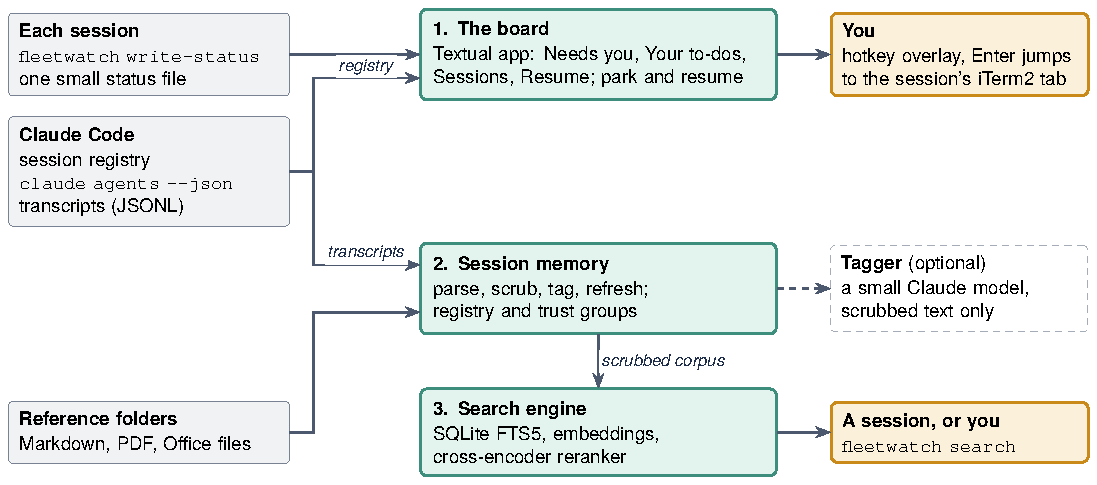
\includegraphics[width=\linewidth, alt={Architecture diagram. Three inputs on the left:
    each session, which writes one small status file with fleetwatch write-status; Claude
    Code, which provides the session registry, claude agents --json and the transcripts; and
    reference folders of Markdown, PDF and Office files. The status file and the registry
    feed layer 1, the board, a Textual app with the tabs Needs you, Your to-dos, Sessions,
    Resume and Indexes, which feeds you through the hotkey overlay, where Enter jumps to a session's
    iTerm2 tab. Transcripts and reference folders feed layer 2, session memory, which parses,
    scrubs, tags and refreshes, and keeps the registry and trust groups. It sends scrubbed
    text to an optional tagger, a small Claude model, and passes a scrubbed corpus to layer
    3, the search engine: SQLite FTS5, embeddings and a cross-encoder reranker, which answers
    fleetwatch search for a session or for you.}]{architecture}
  \caption{The three layers, what each reads, and who uses what it produces.}
  \label{fig:architecture}
\end{figure}

Everything lives in ordinary folders under the home directory. Settings, groups, parked notes
and the index registry are in \cmd{\textasciitilde/.config/fleetwatch}; status files in
\cmd{\textasciitilde/.claude/state/fleetwatch}; each index's corpus and search database in
\cmd{\textasciitilde/.local/share/fleetwatch/indexes/<name>}; logs in
\cmd{\textasciitilde/.local/state/fleetwatch}. Each can be moved with an environment
variable or a setting.

\section{Session memory}

Compaction keeps a session going past the length of its context, and it drops detail to do
it. The decision made on Tuesday and the reason for it are in the transcript, but no longer in
the session's head. A session index puts them back within reach.

From inside a session, one command registers it:

\begin{code}
\begin{verbatim}
fleetwatch index add --group work --docs ~/notes/billing --include '**/*.md'
fleetwatch index refresh
\end{verbatim}
\end{code}

\cmd{index add} finds every project folder that holds the session's transcripts (a session
that moved repositories has more than one), writes a registry entry, and leaves three
templates to edit: the tag taxonomy, the probe questions used to measure search quality, and
the scrub allowlist. \cmd{--docs} adds a reference folder. \cmd{index refresh} reads what is
new, splits the transcript into exchanges (my message and the reply), scrubs them, tags
them, and rebuilds the search database when something changed.

Then the session, or I, can ask:

\begin{code}
\begin{verbatim}
$ fleetwatch search "refund approver"
 1. [bm25 3.0952 ] L20261111 area -    owner    S5e5510-EX-0002.owner.md
    S5e5510-EX-0002 session reply Done. The [refund] service now holds any
    [refund] over 500 dollars until a second [approver] signs off, ...
\end{verbatim}
\end{code}

Without \cmd{--index}, \cmd{search} uses the calling session's own index, found the same way
\cmd{write-status} finds the session. Plain keywords use full-text ranking. \cmd{--similar}
is for a question in ordinary words: it adds embedding search and a reranker, so ``why did
the export break'' finds ``the export ran out of disk on the worker''. \cmd{search show ID
--around 2} prints an exchange with the two on either side, and \cmd{--kind}, \cmd{--tag} and
\cmd{--json} narrow and format the results.

A few details make the index trustworthy over months:

\begin{itemize}
  \item \textbf{Senders are kept apart.} Each exchange records who sent the message: me, a
    scheduled heartbeat, a subagent, another session. A search for what I decided can leave
    out what a timer said (\cmd{--kind '!heartbeat'}). One-shot automated runs are skipped
    entirely.
  \item \textbf{Reference folders and filing.} A folder registered with \cmd{--docs} is
    converted to Markdown and scrubbed like the transcript: Markdown and text as they are, PDF
    through \cmd{pdftotext}, Word and other rich text through \cmd{pandoc}, slides and
    spreadsheets through their Python readers or LibreOffice. When a session files a new
    document, \cmd{fleetwatch index file PATH} indexes it at once, without waiting for the
    next refresh.
  \item \textbf{Tagging is optional.} A tagging pass sends each new exchange, already
    scrubbed, to a small Claude model through \cmd{claude -p} (Haiku by default). It adds an
    area, one to three kinds (such as decision, question or finding), topics and a one-line
    summary, from the taxonomy in the index's \cmd{tags.yaml}. Tags are cached by a hash of
    the exchange, so each one is tagged once, and a run tags at most 400, newest first.
    \cmd{--no-tag} skips it.
  \item \textbf{History is kept.} Claude Code removes old transcripts after a while. An index
    keeps a deleted transcript's exchanges unless its entry says \cmd{on\_missing: remove},
    and \cmd{fleetwatch index forget NAME SESSION\_ID} takes one session out on purpose.
  \item \textbf{It refreshes itself.} \cmd{fleetwatch index schedule install} writes a
    launchd agent on macOS, or a systemd user timer elsewhere, that refreshes every index
    every 30 minutes at low priority. It prints the command that starts it and does not
    start it.
  \item \textbf{Numbers, not text, for health.} \cmd{fleetwatch index verify NAME} reports
    counts, checksums and the search score on the probe questions, and never prints corpus
    text, so its output can be shared without showing what the index holds.
\end{itemize}

\section{Privacy and trust}

Transcripts hold everything that passed through a session: names, email addresses, the odd
pasted key. Nothing is written to an index until it has been scrubbed, and nothing reaches
the tagger that was not scrubbed first. Figure~\ref{fig:scrub} shows a fictional message
before and after.

\begin{figure}[htbp]
\begin{code}
\begin{verbatim}
Sent:    Send the vendor contract to Jordan Lee at jordan.lee@example.com or
         call 303-555-0142. The vendor login is user 4471923 and the key is
         sk-ant-api03-AbCd...(a fictional key)
Stored:  Send the vendor contract to [name] at [email] or call [phone]. The
         vendor login is user [id] and the key is [secret].
\end{verbatim}
\end{code}
  \caption{What the scrubber keeps. The index records how many of each category it replaced,
    never the values.}
  \label{fig:scrub}
\end{figure}

The scrubber combines patterns with spaCy's English name recognizer. A core rule set is
always on: secrets and keys, email addresses, phone numbers, numbers beside an id word
(``user 4471923''), and person names. Rule packs add to it. One pack ships with fleetwatch,
\cmd{education}, which knows the id words of student systems; my own packs are YAML files in
my config folder and never enter the repository. A pack can define id patterns, anonymous-id
formats with a rule that drops any exchange pairing one with a name, private paths to flag,
and spreadsheet columns to drop on conversion. Each index has an allowlist for the addresses
and names that may stay (colleagues, project names that look like people) and a denylist
stored as hashes, so the names it holds are never written to disk.

The name scrub catches the names spaCy recognizes, and spaCy misses some. An all-capital
surname is redacted when it sits beside a name in normal case, a title or a roster comma
(``Jean DUPONT'', ``DUPONT, Jean''), is on the 2010 US Census surname list, and is not a
known acronym, so ``Claude API'' stays. A name wholly in capitals, an all-capital surname on
its own, and a surname that is also a common acronym are left alone. Where names must stay
out of an index, give the index a denylist, which matches a name in any case.

\subsection{Trust groups}

Every index belongs to a group, such as \cmd{work}, \cmd{research} or \cmd{personal}, and the
registry says which groups may read which. A session's own group is the group of its own
index. When a session runs \cmd{fleetwatch search --index X}, fleetwatch checks that its group
is among X's readers, or that the session is named in X's \cmd{extra\_readers}, and otherwise
refuses and names the rule:

\begin{code}
\begin{verbatim}
fleetwatch search: refused: index 'advising-desk-session' is in the
protected group 'ferpa', which only its owner session and the sessions in
its extra_readers may read; group readers never apply.
\end{verbatim}
\end{code}

A \emph{protected} group is stricter. Its name comes from FERPA, the United States law on
student records, and it is the default protected group; \cmd{settings.toml} can name others.
A protected index is readable only by the session that owns it and any session the owner
lists, whatever the group's readers say. It also refuses to start until the rule packs define
id patterns and anonymous-id rules, and it refuses the allowlist options that would scrub
less. Every \cmd{index} command that names an index runs the same check, and \cmd{index
status} lists only what the calling session may read. At a plain terminal, outside any
session, I am the owner and may read everything.

This is a guard against mistakes, not a security boundary. The index files are ordinary
files that anyone with my account can read. What it prevents is the realistic failure: a
session working on one project searching its way into another project's records because a
search returned them.

\section{The search engine as a library}\label{sec:library}

The engine under \cmd{fleetwatch search} is a library, \cmd{fleetwatch.search.engine}, that
works on any folder of Markdown. An index is a directory with a \cmd{search\_config.yaml}:

\begin{code}
\begin{verbatim}
corpus_root: ~/notes
index_path: .index/notes.sqlite
level_folder_pattern: '^(\d{8})()$'
chunking: {max_chars: 1500, min_chars: 25}
similarity:
  model: sentence-transformers/all-MiniLM-L6-v2
  window_chars: 1200
  window_overlap: 300
  rrf_k: 60
roots:
  - {name: notes, path: ., default_kind: note}
\end{verbatim}
\end{code}

\begin{code}
\begin{verbatim}
from fleetwatch.search import engine

ix = engine.Index("myindex")          # the directory holding search_config.yaml
ix.build()
found = ix.search("who signs off on a big refund", similar=True, limit=1)
for row, score in found.results:
    print("%.2f  %s" % (score, row["heading"]))
\end{verbatim}
\end{code}

Each Markdown file is split at its headings into chunks, and each chunk is stored in SQLite
with an FTS5 full-text index and an embedding vector. A keyword search is ranked by BM25. A
similar search runs both, fuses the two rankings by reciprocal rank fusion, and reranks the
top results with a cross-encoder (\cmd{BAAI/bge-reranker-base} by default). The engine
corrects typos against the corpus's own words, expands queries with an optional
\cmd{synonyms.yaml}, and measures itself: \cmd{evaluate()} runs the questions in
\cmd{probes.yaml} and reports the mean reciprocal rank of the expected answer, so a change to
chunking or ranking is judged by a number. The library returns data and raises exceptions; it
never prints or exits. A \cmd{backend: tfidf} setting replaces the embeddings with TF-IDF
vectors for tests and machines without the model libraries.

\section{Setting it up}

fleetwatch needs Python 3.11 or newer. The board runs anywhere Textual does; the overlay and
the jump to a session's tab need macOS and iTerm2.

\begin{enumerate}
  \item \textbf{Install.} The board alone needs no extras. Session memory needs both:
\begin{code}
\begin{verbatim}
pip install 'fleetwatch[search,memory] @ git+https://github.com/daniel-pittman/fleetwatch'
\end{verbatim}
\end{code}
    From a checkout, \cmd{pip install -e '.[search,memory]'} does the same.
  \item \textbf{Look first.} \cmd{fleetwatch --demo} shows the board on the fictional fleet.
  \item \textbf{Install the overlay.} \cmd{fleetwatch iterm install}, then Control-Shift-F. If
    the hotkey does nothing, record it once in iTerm2's settings for the \cmd{fleetwatch}
    profile; the README has the steps.
  \item \textbf{Teach your sessions to report.} Add a paragraph like this to
    \cmd{\textasciitilde/.claude/CLAUDE.md}, which every session reads:
\begin{code}
\begin{verbatim}
Report your status by piping JSON to `fleetwatch write-status`: what you are
working on (working_on), the questions waiting on me (questions), and only the
dated things I must do myself (upcoming, with "yours": true and a due date).
Write it whenever your questions change and at the end of any turn that
leaves work running.
\end{verbatim}
\end{code}
  \item \textbf{Give a session a memory.} From inside it, run \cmd{fleetwatch index add
    --group work}, then build it and search it. The first build downloads the embedding model
    and the reranker (about 1.1~GB, once) and says so; after that, models load offline:
\begin{code}
\begin{verbatim}
fleetwatch index refresh --no-tag
fleetwatch search "anything" --similar
\end{verbatim}
\end{code}
    The first \cmd{index add} creates the registry with its group. A second group is declared
    by hand, in \cmd{\textasciitilde/.config/fleetwatch/indexes/registry.yaml}:
\begin{code}
\begin{verbatim}
groups:
  work:     {readers: [work]}
  personal: {readers: [personal, work]}
\end{verbatim}
\end{code}
  \item \textbf{Schedule it.} \cmd{fleetwatch index schedule install}, then run the
    \cmd{launchctl} (or \cmd{systemctl}) command it prints.
  \item \textbf{Settings,} all optional, in \cmd{\textasciitilde/.config/fleetwatch/settings.toml}:
\begin{code}
\begin{verbatim}
timezone = "America/New_York"   # dates on the board and in the index
owner_name = "Sam"              # how transcripts label your messages

[scanner]
rule_packs = ["education", "my-pack.yaml"]

[groups]
protected = ["ferpa"]
\end{verbatim}
\end{code}
\end{enumerate}

\section{Limits}

fleetwatch is a tool I built for my own way of working, and it has edges.

\begin{itemize}
  \item \textbf{It reads Claude Code's internal files.} The session registry, the transcript
    format and \cmd{claude agents --json} are not a published interface, and a Claude Code
    release can change them. When \cmd{claude agents} fails, fleetwatch warns once and carries
    on with the registry, but a changed transcript format needs a fleetwatch update.
  \item \textbf{The overlay and the jump are macOS and iTerm2 only.} The board, the status
    files and session memory run on Linux too; Enter there cannot raise a tab.
  \item \textbf{The board knows what sessions tell it.} Liveness comes from process checks
    and the registry. Questions and dates come from status files, so a session that never
    writes one shows as alive and nothing more.
  \item \textbf{The scrubber is good, not perfect.} Patterns and a name recognizer miss
    things: an unusual name, a key in a format no rule knows. \cmd{fleetwatch index triage
    NAME} lists likely names the allowlist does not cover (counts only), and a protected
    group adds rules, but an index near sensitive records still deserves a human look.
  \item \textbf{Trust groups prevent mistakes, not attacks.} Anything running as my account
    can read the files.
  \item \textbf{The models are large and the tagger is not free.} The first build downloads
    about 1.1~GB of models; after that everything runs offline. Tagging uses model calls on
    your Claude account, which is why it is capped per run and can be turned off.
  \item \textbf{The library wants a full configuration.} The search engine has few defaults,
    so a search configuration needs every key shown in Section~\ref{sec:library}.
  \item \textbf{One machine.} There is no sync. Each machine has its own board and its own
    indexes.
\end{itemize}

fleetwatch is MIT licensed. The README covers every command and setting; CONTRIBUTING
explains how to run the checks, including the rule that tests and docs use fictional names
only; and SECURITY says how to report a problem privately. I would love to hear how it works
for you.

\end{document}
